\documentclass[a4paper,DIV=12,BCOR=7mm,abstract=yes,twoside,11pt]{scrreprt}

\author{Joshua Clark}

\usepackage{amsmath}
\usepackage{amssymb}
\usepackage[citestyle=authoryear]{biblatex}
\usepackage{backnaur}
\usepackage{url}
\usepackage{algorithm2e}
\bibliography{references}
\usepackage{booktabs}
\usepackage{tikz}
\usepackage{multicol}
\usepackage{pdfpages}
\usepackage[kerning=true,tracking=true]{microtype}

\usepackage{graphicx}
\usepackage[unicode=true,bookmarks=true,bookmarksnumbered=false,bookmarksopen=false,breaklinks=true,pdfborder={0 0 0},colorlinks=false]{hyperref}
\hypersetup{pdftitle={E-Mail Header Information}, pdfauthor={Joshua Clark}}

\usepackage{fancyvrb}
\usepackage{listings}
\usepackage{xcolor}
\usepackage{epigraph}
\usepackage{framed}
\usepackage{lmodern}
\usepackage[T1]{fontenc}
\usepackage{chngcntr}
\usepackage{lscape}

\usepackage{filecontents}
\usepackage{pgfplots, pgfplotstable}
\usepgfplotslibrary{statistics}
\usetikzlibrary{arrows.meta}

\definecolor{mygreen}{rgb}{0,0.6,0}
\definecolor{mygray}{rgb}{0.5,0.5,0.5}
\definecolor{mymauve}{rgb}{0.58,0,0.82}

\lstset{ %
  backgroundcolor=\color{white},   % choose the background color
  basicstyle=\small\ttfamily,      % size of fonts used for the code
  breaklines=true,                 % automatic line breaking only at whitespace
  captionpos=b,                    % sets the caption-position to bottom
  commentstyle=\color{mygreen},    % comment style
  keywordstyle=\color{blue}\bfseries,       % keyword style
  stringstyle=\color{mymauve}\itshape,     % string literal style
  columns=flexible
}


\usepackage{listings}
\lstnewenvironment{example}[1][]{
    \renewcommand*{\lstlistingname}{E-Mail Header Fragment}
    \lstset{fancyvrb=true,basicstyle=\small\ttfamily,captionpos=b,columns=flexible,escapeinside=||,#1}
}{}

\begin{filecontents}{data.csv}
data
0.594924812
0.448717949
0.584134615
0.559210526
0.609601449
0.598557692
0.601190476
0.657738095
0.580357143
0.679761905
0.635416667
0.645833333
0.591666667
0.629807692
0.45
0.604166667
0.651785714
0.5
0.636111111
0.5375
0.583333333
0.605392157
0.541666667
0.61622807
0.558333333
0.528409091
0.588888889
0.541666667
0.583333333
0.614583333
\end{filecontents}

\allowdisplaybreaks{}

\counterwithout{figure}{chapter}
\counterwithout{table}{chapter}

\pagenumbering{roman}
\begin{document}

\thispagestyle{empty}

\begin{center} \begin{minipage}[c]{0.75\linewidth} \centering %University

\includegraphics[width=0.4\linewidth]{oxford}

\vspace{2cm} %Thesis title
{\uppercase{\Large{}Understanding Information\\Leakage in E-Mail Headers}{\Large \par}} \vspace{2cm}
%Author's name
{\Large{}Joshua Clark}{\Large \par}

\vspace{2cm} %Degree
{\Large{}Fourth Year Project Report for the Final Honour School of
Computer Science}{\Large \par}

\vspace{2cm} %Date
{\Large{}May 2016} %
\end{minipage} \par\end{center}

\cleardoublepage 
\chapter*{Abstract}

After extensive public education, fewer people are now clicking on links in
e-mails that are disguised as phishing attacks, though the threat still
remains, and a considerable amount of work has gone into exploring the
demographics most likely to be targeted.  As the number of technically literate
people grows, this sort of attack is less frequently successful.
Therefore, malicious entities are more likely to attempt to attack people based
on the information leaked in their emails, and more specifically, the header,
which most people will not have a degree of control over.

The risks are not just limited to individual users, and at a corporate level,
the risks posed by leaking information through e-mails could be even greater:
e-mail headers can reveal the internal network structure of a company's
computer systems as well as the different pieces of software that are running
inside the system.  Extracting the social information could be of great value
for executing a phishing attack, however, there is also value in determining
the specific weaknesses in a system.  This can be aided through the use of
vulnerability databases.

This report discusses the existing research into the information leaked by
e-mail headers and presents a tool to extract such information.  The tool's
design and implementation is discussed, followed by the results of its testing.

\cleardoublepage 
\chapter*{Acknowledgements}

I want to thank my supervisor, Dr Jason R.C. Nurse for his assistance
throughout the year; my tutor, Professor Peter Jeavons, for his unfailing
help and support throughout my time at Oxford.  I would like to thank the
residents and chaplains of the Oxford University Catholic Chaplaincy.
Finally, I would like to acknowledge the support from my family and
partner, Agata Borkowska, for encouraging me.

\cleardoublepage 
\tableofcontents 
\clearpage
\let\LaTeXStandardClearpage\clearpage
\let\clearpage\relax  % Do nothing when a \clearpage command appears 

\listoftables \listoffigures \listofalgorithms

\let\clearpage\LaTeXStandardClearpage % Return to the old definition


\cleardoublepage 
\chapter{Introduction}\label{chap:int}
\pagenumbering{arabic}
\setcounter{page}{1}

\section{Motivation}

E-mail systems are now so integrated into our modern lives that we struggle to
cope without them.  E-mails ubiquity is also one of its largest weaknesses, a
fact recognised very early on.  The first spam email was sent in 1978, as
documented by~\cite{templeton}.  After spam came phishing, first described
by~\cite{felix1987system}, with the first-real world use being against the
customers of America Online, an ISP.\@  However, this still relies on the
targets providing their data for malicious purposes. One of the first e-mail
viruses to spread was the Happy99 virus, which, other than propagating itself,
had no effect on infected systems. Later viruses would target credit-card and
banking information. However, all of these techniques rely on the malicious
email being received and its contents being opened.  There are fewer instances
recorded, however, of the information flow being sent the other way.  A more
subtle attack will focus on the information being sent from a legitimate user
to an attacker. It is easy enough for an individual to read an e-mail header
and identify interesting elements, however, on a large scale, this quickly
becomes more difficult.

\section{Aims and Objectives}

This project aims to support a better understanding of the data that may be
leaked when e-mails are sent, both from a personal perspective, as well as the
corporate data that is disclosed concerning network configurations and software
installations.

To support this, I will develop a tool that can be used as described above to
automatically extract information from e-mail headers and analyse its results to
display the personal information contained within an e-mail's header, as well as
information about the software configurations that may be found on a user's
computer, or the servers used to send their e-mail.

The tool's objectives will be to parse, analyse and visualise the contents of
any e-mail header that it is given.  The parsing process should correctly and
efficiently convert the plaintext of an e-mail header into an abstract
representation.  In the analysis section, the representation of the header
should be searched to find information out about the sender, their software and
device, and information for any servers that the e-mail message passes through.
Finally, the visualisation produced should clearly show the information that is
available about the sender of an e-mail and the path the e-mail took in order to
arrive at its final destination.

\section{Structure}

Chapter~\ref{chap:exres} begins by discussing the existing research on
the subject as well as existing publicly-available tools to analyse
headers.  I then use these as a basis to discuss features that would be
expected to appear in a header analyser looking for leaked information
and vulnerabilities.

The specification and design of a program to support the understanding of the
information leaked in e-mail headers is discussed in Chapter~\ref{chap:des}.
The implementation's high-level structure and details will be discussed in
Chapter~\ref{chap:imp}, and algorithms presented in pseudo-code where
necessary.  A full listing will be presented at the end of this document in
an appendix. The results of the analysis of the headers will be discussed in
Chapter~\ref{chap:test}, beginning with the methodology used, and presenting
a number of results, finishing with conclusions and areas for improvement.

\cleardoublepage \chapter{Existing Research}
In \cite{nurse2015investigating}, the idea of using the information available in an email header was mooted, turning the previously standard threat of malware and phishing contained in received e-mails on its head, and instead presenting the threat in outgoing emails, and the personally identifying information (PII) contained therein.  Many emails leaked information about employers, e-mail services and applications used, and IP address.  Initial examination of a variety of e-mail headers found within my own inbox also revealed a plethora of information, including phone carriers, preferred languages, and system usernames.  It is conceivable therefore, that it is possible to automate at least part of this, and present the information that can be extracted, in a white-hat tool to allow people to audit the information that they are revealing.  The obvious malicious use-case involves using such information as part of a spear-phishing exercise.

An alternative vulnerability presents itself in the information about systems that may be revealed.  Many email clients embed identifying information, and there are multiple databases available to allow specific threats to be identified.  This could allow a malicious entity to compromise the security of a target machine, and gain access to the data stored on that machine and available on any connected network devices.  Work started in \cite{joshi2013extracting} discusses the need to aggregate data about vulnerabilities from multiple sources to present a more complete and coherent picture, which is also likely to then contain more accurate data.

\cite{Al-zarouni_tracinge-mail} presents an alternative set of results, describing how an individual can seek to protect themselves against malicious e-mails, using the contents of e-mail headers.  Various discrepancies between forged e-mail addressses and legitimate messages are described. 
\cleardoublepage \chapter{Design}
\section{Requirements}
The program would be expected to satisfy the following minimal requirements
in order for it to be considered successful: 
\begin{description}
\item [{Accuracy}]  -- any information produced by the parser should be reflective of the input e-mail
\item [{Representation}] -- the produced visualisation should be intuitive to read: each element should be presented separately from the others, and clearly labelled. 
\item [{Portability}] -- the visual output produced by the program should be available to the user in a variety of formats. 
\item [{Interactivity}] the program should produce sensible warnings when
an e-mail that is not possible to parse has been entered. 
\end{description}

 
\cleardoublepage \chapter{Implementation}\label{chap:imp}
\section{Overview}

The  analysis is implemented as a series of stages, firstly, the e-mail header
is parsed, to extract important information to a predefined set of Java objects.
This is followed by the analysis phase, where the resultant data is passed to a
set of analyser modules, each running separately.  Finally, this information is
presented to the user.  This chapter presents each of these stages in detail.

\section{Definitions}

The following covers the essential definitions required for the notation and
concepts that will be discussed in this document.

\subsection{Parsing}

In order to aid the parsing of the e-mail header, a combination of regular
expressions and context-free grammars are needed, and defined as follows.

\paragraph{Alphabets and Languages}

A set of symbols, usually denoted as $\Sigma$.  A language is a subset of
$\mathcal P (\Sigma)$.

The following special classes are provided as part of the Perl-Compatible
Regular Expression library, and are subsets of the alphabet of Unicode
characters, defined in~\cite{php_group_gutmans_lerdorf_suraski_boerger}.

\begin{description}

\item[alnum] --- letters and digits

\item[alpha] --- letters

\item[ascii] --- the set of ASCII characters (character codes 0 --- 127)

\item[blank] --- tabs or blank spaces

\item[cntrl] --- control characters

\item[digit] --- decimal digits

\item[graph] --- printing characters (excluding spaces)

\item[lower] --- lower-case letters

\item[print] --- printing characters (including spaces)

\item[punct] --- punctuation marks (printing characters excluding letters and spaces)

\item[space] --- white space

\item[upper] --- upper case letters

\item[word] --- ``word'' characters (same

\item[xdigit] --- hexadecimal digits

\end{description}
\subsubsection{Regular Languages}
Regular languages are defined as follows:
\begin{itemize}
\item $\emptyset$ and $\{\epsilon\}$ are regular languages
\item for each $a\in\Sigma$, $\{a\}$ is a regular language
\item if $A$ and $B$ are both regular, $A\cup B$, $A\cdot B$ and $A^*$ are regular languages.
\subitem{ $A\cup B$ is the union of two languages.  $A\cup B = \{s : s\in A \lor s \in B\}$}
\subitem{ $A\cdot B$ is the concatentation of two languages.  $A\cdot B = \{ ab : a \in A, b \in B\}$}
\subitem{ $A^*$ is the Kleene star of a language.}
\begin{align*}
    A_0&=\{\epsilon\}\\
    A_1&= A\\
    A_{i+1} &= \{ aa' : a \in A_i, a'\in A\}\\
    A^* &= \bigcup_{i\in\mathbb N} A_i
\end{align*}
\end{itemize}

\subsubsection{Context-Free Grammars}
A context-free grammar $G$ is defined as $G=\left(V,\Sigma, R,S\right)$ where:
\begin{itemize}
\item $V$ is a variable.
\item $\Sigma$ is the alphabet of symbols.
\item $R$ is a relation defined over $V\rightarrow \left(V\cup\Sigma\right)^*$
\item $S$ is the start symbol
\end{itemize}

For example, $\langle \text S \rangle$ is the field name with the associated
productions $\langle \text T \rangle \, \langle \text U \rangle$, where $T$ and
$U$ are productions.

\begin{bnf*}
	\bnfprod{S}{\bnfpn{T} \bnfsp{} \bnfpn{U}}
\end{bnf*}

For example, $\langle \text S \rangle$ is the field name with the associated
productions $a \, \langle \text U \rangle$, where $a$ is a terminal symbol.

\begin{bnf*}
	\bnfprod{S}{\bnftd{a} \bnfsp{} \bnfpn{U}}
\end{bnf*}
This is then extended in the following ways used in the RFC syntax.

The square brackets are used to indicate an optional element.
\begin{bnf*}
\bnfprod{field}{\bnfpn{field-name} \bnfts{:} \bnfsp{}[ \bnfpn{field-body} ]\bnfsp{} \bnfts{CRLF}}\\
\end{bnf*}

The asterisk is used to indicate an element that appears 0 or more times. $n*$
is used to indicate a component that repeats $n$ or more times.

\begin{bnf*}
\bnfprod{fields}{\bnfpn{dates}\bnfsp \bnfpn{source} \bnfsp 1\!*\bnfpn{destination} \bnfsp * \bnfpn{optional-fields}}\\
\end{bnf*}

The hash-symbol is used to indicate an element that appears a certain number of
times. $m*n$ is used to indicate a component that repeats at least $m$ times and
at most $n$ times.

\begin{bnf*}
\bnfprod{fields}{\bnfpn{dates}\bnfsp \bnfpn{source} \bnfsp 1\!\#\bnfpn{destination} \bnfsp * \bnfpn{optional-fields}}\\
\end{bnf*}

The $|$ is used to indicate a selection between a pair of elements.
\begin{bnf*}
\bnfprod{fields}{\bnfts{a}\bnfor \bnfts{b}}\\
\end{bnf*}

\subsection{Database Queries}
The following notations will be used for the CVE database queries.

\paragraph{Set-Theoretic Operators}
The operators $F\cup G$, $F \cap G$, $F\setminus G$ behave as is expected for
these operators, resulting in the union, intersection and difference of the
sets.  The only proviso being that the atrribute names must match.

\paragraph{Selection} \[\sigma_{\text{product}=\text{thunderbird}}D\]
The above notation is used to indicate a search over the attribute named
``product'' for the string ``thunderbird'' in the database table $D$.  As a
single database is only being used, this may be occasionally elided.  The output
of this function is another object of the same type as $D$.

\paragraph{Projection}
\[\pi_{\text{product}}D\]
The above notation is used to indicate a projection on the attribute named
``product'' in the database table $D$.  The output of this function is another
object of the same type as $D$.

\paragraph{Composition}
The above functions results can be coposed repeatedly to produce more specific
search queries.

\section{Data Extraction and Parsing}

The parser's operation completes in a number of stages, following RFC822
(\cite{RFC0822}).  The header is divided up into two disjoint sections, the
routing information (\texttt{Received from...}) and the key-value map of other
pertinent information.

\subsection{Received fields}

The received fields are the most complicated part of the e-mail header to parse,
as they are described by a non-trivial grammar, presented below.

\begin{bnf*}
\bnfprod{message}{\bnfpn{fields}\bnfsp *(\bnfts{CRLF} \bnfsp *\bnftd{text})}\\
\bnfprod{fields}{\bnfpn{dates}\bnfsp \bnfpn{source} \bnfsp 1\!*\bnfpn{destination} \bnfsp * \bnfpn{optional-fields}}\\
\bnfprod{field}{\bnfpn{field-name} \bnfts{:} \bnfsp [ \bnfpn{field-body} ]\bnfsp \bnfts{CRLF}}\\
\bnfprod{field-name}{\bnftd{any word consisting of CHAR, excluding CTLs, SPACE, and ``'':''}} \\
\bnfprod{field-body}{\bnfpn{field-body-contents} \bnfsp [\bnfts{CRLF} \bnfsp \bnftd{LWSP-char}\bnfsp  \bnfpn{field-body}]}\\
\bnfprod{field-body-contents}{\bnftd{ASCII characters}}\\
\bnfprod{source}{[\bnfpn{trace}] \bnfsp \bnfpn{originator} [\bnfpn{resent}]}\\
\bnfprod{trace}{\bnfpn{return}\bnfsp 1\!* \bnfpn{received}}\\
\bnfprod{return}{\bnfts{Return-path:}\bnfsp{} \bnfpn{route-addr}}\\
\bnfprod{recieved}{\bnfts{Received:}}\\
\bnfprod{cont.}{[\bnfts{from}\bnfsp\bnfpn{domain}]}\\
\bnfprod{cont.}{[\bnfts{by}\bnfsp\bnfpn{domain}]}\\
\bnfprod{cont.}{[\bnfts{via}\bnfsp\bnfpn{atom}]}\\
\bnfprod{cont.}{*(\bnfts{with}\bnfsp\bnfpn{atom})}\\
\bnfprod{cont.}{[\bnfts{id}\bnfsp\bnfpn{msg-id}]}\\
\bnfprod{cont.}{[\bnfts{for}\bnfsp\bnfpn{addr-spec}]}\\
\bnfprod{cont.}{\bnfts{;}\bnfsp\bnfpn{date-time}}\\
\bnfprod{msg-id}{\bnfts{$<$}\bnfpn{addr-spec}\bnfts{$>$}}\\
\bnfprod{addr-spec}{\bnfpn{local-part}\bnfsp\bnfts{@}\bnfsp\bnfpn{domain}}\\
\bnfprod{local-part}{\bnfpn{word}\bnfsp *(\bnfts{.}\bnfsp\bnfpn{word})}\\
\bnfprod{word}{\bnfpn{atom}\bnfor\bnfpn{quoted-string}}\\
\bnfprod{domain}{\bnfpn{sub-domain} *(\bnfts{.}\bnfpn{sub-domain})}\\
\bnfprod{sub-domain}{\bnfpn{domain-ref}\bnfor\bnfpn{domain-literal}}\\
\bnfprod{domain-ref}{\bnfpn{atom}}\\
\bnfprod{date-time}{[ \bnftd{day,} ] \bnfsp \bnftd{date}\bnfsp \bnftd{time}}\\
\bnfprod{atom}{1\!*\bnftd{any character excluding specials, SPACE and CTLs}}\\
\end{bnf*}

An example field is as follows:
\begin{verbatim}
Received: from relay12.mail.ox.ac.uk (129.67.1.163)
    by HUB05.ad.oak.ox.ac.uk (163.1.154.231)
    with Microsoft SMTP Server id 14.3.169.1;
    Sat, 14 Nov 2015 10:55:35 +0000
\end{verbatim}
\subsection{Other fields}

These are read by a Python script and output to \texttt{STDOUT} to be read by
the Java parser in a consistent format.  These are then loaded into a hashmap to
allow quick lookup.

\section{Analysis}

After completing the parsing of the field, it is then ready to be analysed for
different features.  All of the analysers implement the \texttt{HeaderAnalyser}
interface, requiring information about the header to be analysed, and the
currently running application.  All of these then implement the
\texttt{Runnable} interface, allowing the class to be run asynchronously.

\subsection{Text-Based}

The fields from the header are analysed in different modules, with searches
being performed for specific strings.  Of particular interest to Oxford Nexus
users is the ``X-Oxford-Username'' string, containing the username of the
individual that sent the message.  As confirming the username is a fairly
standard security procedure for an IT support technician, having access to this
information could allow a phisher in a later stage of an attack to increase
their credibility.

In some cases, the likely keys that are being searched for are known in advance,
and can then be checked against the hash-map of entries.

An example of this approach is for the specific check for an Oxford username:

\begin{algorithm}
	\KwIn{Header}
	\KwOut{Any Oxford-based username that is found}
	\If{\texttt{X-Oxford-Username} $\in$ Header.KvMap}{ \Return{Header.KvMap(X-Oxford-Username)}\; }
	\caption{Lookup based on a known key}
\end{algorithm}

Alternatively, we may be interested in properties of the keys, necessitating a search over the keys.

\begin{algorithm}
	\KwIn{Header}
	\KwOut{Any information relating to Microsoft Exchange that is found}
	\ForEach{Key $k\in $ Header.KvMap}{
		\If{$k$ starts-with \texttt{X-MS-Exchange}}{
			\Return{Header.KvMap($k$)}\;
		}
	}
	\caption{Lookup based on a key property}
\end{algorithm}

\subsection{Database Queries}

Using the results gathered from the text-based queries and analysis of the
received fields, relevant software configurations are extracted and queried
against results in the CVE database.  These are then parsed and collated in
preparation for displaying the outputs.

As more information is found, more details of products used will also become
available.  These are added asynchronously.

\begin{algorithm}
	\KwIn{Header product name $p$}
	\KwOut{CVE Entries}
	cve-list $\gets\emptyset$\;
	\ForEach{$s\in\sigma_{\text{vector}\neq\text{LOCAL}}\sigma_{\text{product}=p} D$}{
		cve-builder$\gets$blank cve\;
		cve-builder.id$\gets\pi_{\text{CVE-ID}} s$\;
		$\ldots$ -- extract other features\;
		cve-list $\gets$ cve-list${}\cup{}$make(cve-builder)\;
	}
	\Return{cve-list}\;
	\caption{Extracting CVE entries}
\end{algorithm}

\section{Visualising the Results}

Using a pre-existing template, the results from the e-mail analysis will be
presented in a temporary webpage, which can then be saved independently.  Other
than the referenced JavaScript libraries, the document requires no additional
information or database access, allowing it to be quickly shared.

\cleardoublepage \chapter{Evaluation}\label{chap:test}
After producing the application described in Chapter~\ref{chap:imp}, referring
back to the design specifications to determine its performance against the
stated criteria was the next step.  

\section{Methodology}
Using a sample of e-mails provided by my supervisor, each of them was run
through the final version of the program, and scored based on the following
attributes:

\begin{itemize}
\item Let $M$ be the total number of received fields.
\item Let $N$ be the total number of other fields.
\item 1 point is added to the total $R$ for each piece of information found in a Received field for the following:
\subitem{One of device name \emph{or} IP address}
\subitem{Software \emph{or} protocol used}
\subitem{Vulnerabilities found for the relevant piece of software}
\subitem{Location Data}
\item 1 point is addded to $F$ for each piece of information found in other fields.
\end{itemize}

The final score for an e-mail is given as \[\frac12\left(\frac R{4M}+\frac
FN\right)\]to give a value between 0 and 1 for each e-mail.

The e-mails received have been numbered from 1 up to 70, and a random sample of
size 30 was selected using the following code:

\begin{verbatim}
>>> random.seed()
>>> random.sample(list(range(1,70)), 30)
[64, 48, 11, 21, 63, 68, 27, 69, 29,  8, 28,
 34, 13, 57, 10,  3, 22, 32, 23, 49, 26, 45,
 19,  1, 36, 46, 41, 18, 20, 17]
\end{verbatim}

Thus giving a sorted list of the following e-mails: 1, 3, 8, 10, 11, 13, 17,
18, 19, 20, 21, 22, 23, 26, 27, 28, 29, 32, 34, 36, 41, 45, 46, 48, 49, 57, 63,
64, 68, 69.

\section{Sample Output}

The following pages show the results of running the completed software on the
e-mail labelled \texttt{11.txt}, the contents of which is listed in
Fragment~\ref{eg:11}.  The full table of CVE entries is elided for brevity.  
The entries in \colorbox{red!30}{this colour} are associated with points scored
for $R$, and the entries in \colorbox{blue!30}{this colour} are associated with
points scored for $F$.

\begin{example}[caption=Email \texttt{11.txt},label=eg:11]
Received: from relay13.mail.ox.ac.uk (129.67.1.163) by HUB01.ad.oak.ox.ac.uk 
 (|\colorbox{red!30}{163.1.154.218}|) with |\colorbox{red!30}{Microsoft SMTP Server}| id 14.3.169.1; Wed, 1 Apr 2015 
 11:06:18 +0100 
Received: from postie2.cs.ox.ac.uk ([129.67.151.44])	by |\colorbox{red!30}{relay12.mail.ox.ac.uk }|
 with |\colorbox{red!30}{esmtp (Exim 4.80}|)	(envelope-from <ahayes@mays.tamu.edu>)	id 
 1YdFXO-0008P8-de	for cccc1111@nexus.ox.ac.uk; Wed, 01 Apr 2015 11:06:18 +0100 
Received: from mailer.cs.ox.ac.uk ([129.67.151.81]:36787)	by 
 |\colorbox{red!30}{postie2.cs.ox.ac.uk}| with |\colorbox{red!30}{esmtp (Exim 4.72)}|	(envelope-from 
 <ahayes@mays.tamu.edu>)	id 1YdFWT-0004Fk-DZ	for jason.nurse@cs.ox.ac.uk; Wed, 
 01 Apr 2015 11:05:21 +0100 
Received: from relay11.mail.ox.ac.uk ([129.67.1.162]:57950)	by 
|\colorbox{red!30}{mailer.cs.ox.ac.uk}| with |\colorbox{red!30}{esmtp (Exim 4.72)}|	(envelope-from 
 <ahayes@mays.tamu.edu>)	id 1YdFWS-0003OY-6C	for jason.nurse@cs.ox.ac.uk; Wed, 
 01 Apr 2015 11:05:20 +0100 
Received: from mailbox2.mbs.tamu.edu ([128.194.216.125])	by 
|\colorbox{red!30}{relay11.mail.ox.ac.uk}| with |\colorbox{red!30}{esmtp (Exim 4.80)}|	(envelope-from 
 <ahayes@mays.tamu.edu>)	id 1YdFWS-0000Ck-Zf	for jason.nurse@cs.ox.ac.uk; Wed, 
 01 Apr 2015 11:05:20 +0100 
Received: from MAILBOX1.mbs.tamu.edu ([|\colorbox{red!30}{169.254.2.132}|]) by
MAILBOX2.mbs.tamu.edu ([|\colorbox{red!30}{169.254.1.80}|]) with |\colorbox{red!30}{mapi}| id 14.03.0224.002; Wed, 1
Apr 2015 05:05:00 -0500
From: |\colorbox{blue!30}{"Hayes, Allison" <ahayes@mays.tamu.edu>}|
To: "Hayes, Allison" <ahayes@mays.tamu.edu>
Subject: RE: ITS HELP DESK
Thread-Topic: ITS HELP DESK
Thread-Index: AdBsXNo2iPt2JIAvQzCkSflypfIvlgABOhlv
Date: Wed, 1 Apr 2015 10:04:57 +0000 
Message-ID: <3AC6BF6FEAFA734A8A0397E31CB7AD009B695F@MAILBOX1.mbs.tamu.edu> 
References: <3AC6BF6FEAFA734A8A0397E31CB7AD009A5A35@MAILBOX1.mbs.tamu.edu> 
In-Reply-To: <3AC6BF6FEAFA734A8A0397E31CB7AD009A5A35@MAILBOX1.mbs.tamu.edu> 
|\colorbox{blue!30}{Accept-Language: en-US }|
Content-Language: en-US 
X-MS-Has-Attach: 
X-MS-TNEF-Correlator: 
x-originating-ip: [208.76.111.246] 
Content-Type: multipart/alternative; 
	boundary="_000_3AC6BF6FEAFA734A8A0397E31CB7AD009B695FMAILBOX1mbstamued_" 
MIME-Version: 1.0 
X-Oxmail-Spam-Status: score=2.9 tests=HTML_MESSAGE,SUBJ_ALL_CAPS,T_RP_MATCHES_RCVD,URI_HEX 
X-Oxmail-Spam-Level: ** 
Return-Path: ahayes@mays.tamu.edu 
|\colorbox{blue!30}{X-MS-Exchange-Organization-AuthSource: HUB01.ad.oak.ox.ac.uk }|
|\colorbox{blue!30}{X-MS-Exchange-Organization-AuthAs: Anonymous }|
|\colorbox{blue!30}{X-MS-Exchange-Organization-AVStamp-Mailbox: Sophos;-2052447998;0;PM }|
|\colorbox{blue!30}{X-MS-Exchange-Organization-SCL: 2 }|
\end{example}

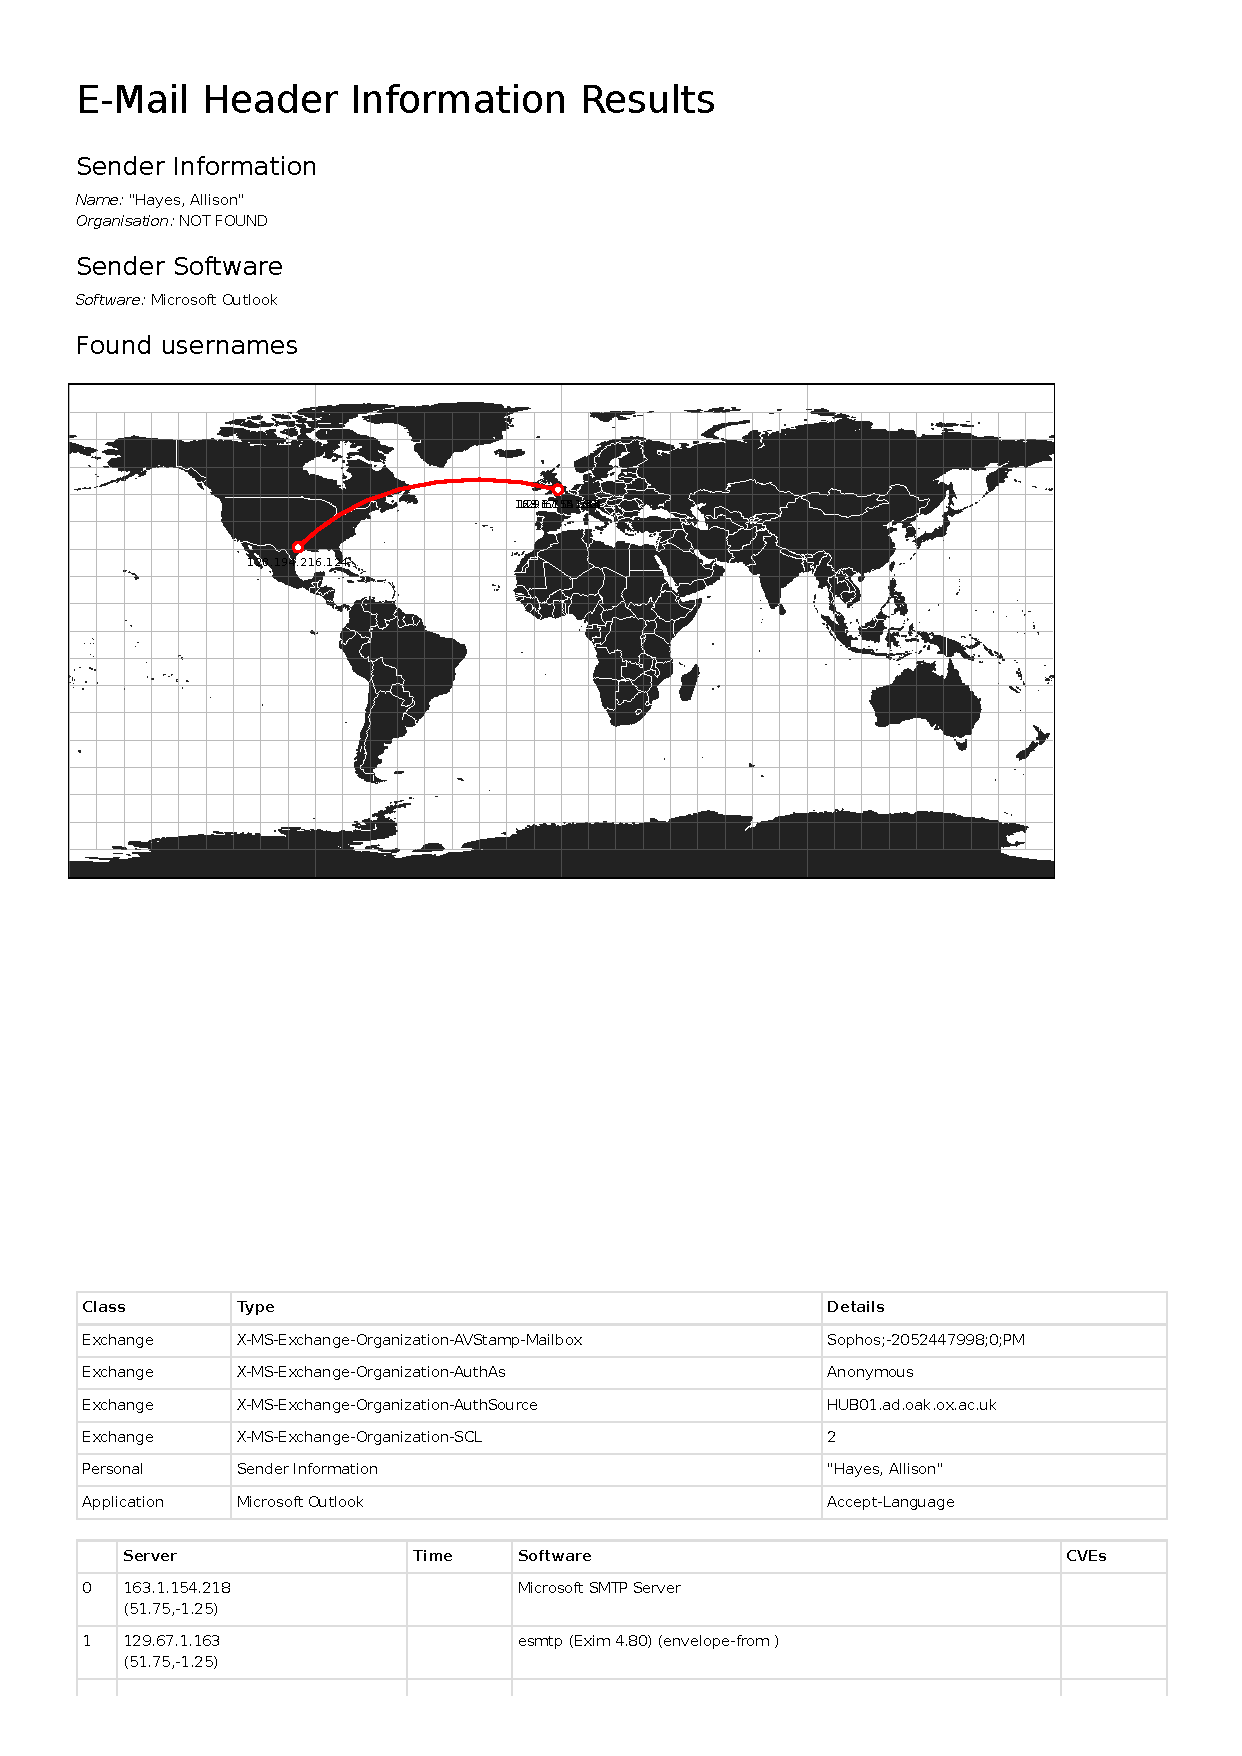
\includepdf[pages={1,2,3}]{11_results.pdf}

\section{Results}

Table~\ref{tab:sammn} gives the $M$ and $N$ values for the different sampled
e-mails.  These were sampled using standard Unix tools: \texttt{grep}ping for
fields and counting the output.

\begin{table}[]
\centering
\begin{tabular}{@{}lccclll@{}}
\toprule
Header & Total Fields &                  $M$  & $N$  & $R$ & $F$ & $S$ \\ \midrule
1.txt  & 26           & 7                     & 19   & 23  & 7   &     \\
3.txt  & 32           & 6                     & 26   & 16  & 6   &     \\
8.txt  & 34           & 8                     & 26   & 30  & 6   &     \\
10.txt & 22           & 3                     & 19   & 9   & 7   &     \\
11.txt & 29           & 6                     & 23   & 23  & 6   &     \\
13.txt & 17           & 4                     & 13   & 13  & 5   &     \\
17.txt & 27           & 6                     & 21   & 22  & 6   &     \\
18.txt & 20           & 6                     & 14   & 23  & 5   &     \\
19.txt & 20           & 6                     & 14   & 21  & 4   &     \\
20.txt & 22           & 7                     & 15   & 25  & 7   &     \\
21.txt & 22           & 6                     & 16   & 23  & 5   &     \\
22.txt & 22           & 6                     & 16   & 22  & 6   &     \\
23.txt & 26           & 6                     & 20   & 20  & 7   &     \\
26.txt & 19           & 6                     & 13   & 21  & 5   &     \\
27.txt & 21           & 1                     & 20   & 2   & 8   &     \\
28.txt & 22           & 6                     & 16   &     &     &     \\
29.txt & 20           & 6                     & 14   &     &     &     \\
32.txt & 24           & 6                     & 18   &     &     &     \\
34.txt & 23           & 5                     & 18   &     &     &     \\
36.txt & 26           & 6                     & 20   &     &     &     \\
41.txt & 21           & 6                     & 15   &     &     &     \\
45.txt & 23           & 6                     & 17   &     &     &     \\
46.txt & 26           & 5                     & 21   &     &     &     \\
48.txt & 25           & 6                     & 19   &     &     &     \\
49.txt & 21           & 6                     & 15   &     &     &     \\
57.txt & 28           & 6                     & 22   &     &     &     \\
63.txt & 23           & 5                     & 18   &     &     &     \\
64.txt & 36           & 9                     & 27   & 31  & 6   &     \\
68.txt & 21           & 6                     & 15   &     &     &     \\
69.txt & 22           & 6                     & 16   &     &     &     \\ \bottomrule
\end{tabular}
\caption{$M$, $N$, $R$, $F$ and score values for chosen headers}
\label{tab:sammn}
\end{table}

The results of the testing are contained within Table~\ref{tab:res}, and give a
breakdown for each e-mail's values of $R$ and $F$, as well as the final score.

During the testing, the following trends were noticed.  As many of the e-mails
passed through the same set of servers, as they had been received by an Oxford
e-mail address, the same set of servers were frequently seen, all of which had
associated IP addresses, geolocation data and (except for one server running
Microsoft SMTP Server) CVE data for the running software.  For an e-mail sent
within the University Nexus system, this gives an inflated score, as very few
of the servers are missing information.

The score for the information gathered from fields does not take into account
the number of fields needed to determine or infer a piece of information. For
example, the presence, or absence of multiple fields is required to determine a
piece of information.  Nor does it consider the relative value of a piece of
information, failing to rate the presence of a username above the presence of a
particular piece of software also giving false positives.

However, very few e-mails in the testing population contained fields relating
to usernames (for example, \texttt{X-}$\ldots$\texttt{-User}, \texttt{X-Oxford-Username},
\texttt{X-Authenticated-User}) compared to the result
in~\cite{nurse2015investigating}, which found 14\% of e-mails to contain
usernames as opposed to the 8\% found in the population.

\section{Conclusions}

As described in Chapter~\ref{chap:int}, the aim of this project is to support a
better understanding of the data that may leaked when e-mails are sent, both
from a personal perspective, as well as the corporate data that is leaked
concern network configurations and software installations.

To support this, I have developed a tool that can be used to automatically
extract information from e-mail headers and analyse its results to display the
personal information contained within an e-mail's header, as well as
information about the software configurations that may be found on a user's
computer, or the servers used to send their e-mail.


\section{Future Work}

During the late stages of development and testing, a number of missing features
quickly became apparent. Due to the limited information available, and the
differences in version numbering, a decision was made to search for all
available vulnerabilities for an application, allowing the user to discern
which were most relevant.  Subsequent versions could focus on the different
pieces of version data available.  For example, \texttt{esmtp} frequently
references its version number in the ``Received'' field frequently.

Alternatively, a better picture may be presented by accumulating multiple
e-mails. For example, using the information provided from multiple members of
single organisation, a better picture may be built up of the software used by
the servers, as well as the network configuration.

The application's response times may also be improved by caching some data in
memory, such as WhoIs responses and GeoIP lookups, so that frequently accessed
lookups can be completed more quickly.

Additionally, future testing should take place on a larger dataset, using
e-mails from a wider variety of sources sent to a number of different
recipients.  

Finally, it should be possible for an updated version of this application to
determine which header fields have been added by mail servers within one's own
organisation.  For example, e-mail header fields beginning with
\texttt{X-MS-Exchange} are seen within almost all e-mail messages sent to
recipients within the Oxford domain, adding more false positives to the test
results. While it is possible that other preceding e-mail servers have added
similar fields, in most cases, these entries yielded little useful data.

 
\cleardoublepage \printbibliography{} 
\cleardoublepage 
\appendix
\begin{landscape}\begin{multicols}{2}
\chapter{Code Listings}
\lstinputlisting[breaklines=true, flexiblecolumns=true, basicstyle=\ttfamily\small, language=java]{emailheaderinformation/src/main/java/com/devdaily/system/SystemCommandExecutor.java}
\lstinputlisting[breaklines=true, flexiblecolumns=true, basicstyle=\ttfamily\small, language=java]{emailheaderinformation/src/main/java/com/devdaily/system/ThreadedStreamHandler.java}
\lstinputlisting[breaklines=true, flexiblecolumns=true, basicstyle=\ttfamily\small, language=java]{emailheaderinformation/src/main/java/emailheaderinformation/analysers/ClientInferrer.java}
\lstinputlisting[breaklines=true, flexiblecolumns=true, basicstyle=\ttfamily\small, language=java]{emailheaderinformation/src/main/java/emailheaderinformation/analysers/DeviceAnalyser.java}
\lstinputlisting[breaklines=true, flexiblecolumns=true, basicstyle=\ttfamily\small, language=java]{emailheaderinformation/src/main/java/emailheaderinformation/analysers/ExchangeHeaderAnalyser.java}
\lstinputlisting[breaklines=true, flexiblecolumns=true, basicstyle=\ttfamily\small, language=java]{emailheaderinformation/src/main/java/emailheaderinformation/analysers/GeoIPAnalyser.java}
\lstinputlisting[breaklines=true, flexiblecolumns=true, basicstyle=\ttfamily\small, language=java]{emailheaderinformation/src/main/java/emailheaderinformation/analysers/HeaderAnalyser.java}
\lstinputlisting[breaklines=true, flexiblecolumns=true, basicstyle=\ttfamily\small, language=java]{emailheaderinformation/src/main/java/emailheaderinformation/analysers/NoopVulnerabilityFinderManager.java}
\lstinputlisting[breaklines=true, flexiblecolumns=true, basicstyle=\ttfamily\small, language=java]{emailheaderinformation/src/main/java/emailheaderinformation/analysers/SenderInformationExtractor.java}
\lstinputlisting[breaklines=true, flexiblecolumns=true, basicstyle=\ttfamily\small, language=java]{emailheaderinformation/src/main/java/emailheaderinformation/analysers/UsernameHeaderAnalyser.java}
\lstinputlisting[breaklines=true, flexiblecolumns=true, basicstyle=\ttfamily\small, language=java]{emailheaderinformation/src/main/java/emailheaderinformation/analysers/VulnerabilityAnalyser.java}
\lstinputlisting[breaklines=true, flexiblecolumns=true, basicstyle=\ttfamily\small, language=java]{emailheaderinformation/src/main/java/emailheaderinformation/analysers/VulnerabilityFinderManager.java}
\lstinputlisting[breaklines=true, flexiblecolumns=true, basicstyle=\ttfamily\small, language=java]{emailheaderinformation/src/main/java/emailheaderinformation/analysers/VulnerabilityFinderManagerImpl.java}
\lstinputlisting[breaklines=true, flexiblecolumns=true, basicstyle=\ttfamily\small, language=java]{emailheaderinformation/src/main/java/emailheaderinformation/analysers/WhoIsAnalyser.java}
\lstinputlisting[breaklines=true, flexiblecolumns=true, basicstyle=\ttfamily\small, language=java]{emailheaderinformation/src/main/java/emailheaderinformation/database/DbManager.java}
\lstinputlisting[breaklines=true, flexiblecolumns=true, basicstyle=\ttfamily\small, language=java]{emailheaderinformation/src/main/java/emailheaderinformation/MainWindow.java}
\lstinputlisting[breaklines=true, flexiblecolumns=true, basicstyle=\ttfamily\small, language=java]{emailheaderinformation/src/main/java/emailheaderinformation/model/Access.java}
\lstinputlisting[breaklines=true, flexiblecolumns=true, basicstyle=\ttfamily\small, language=java]{emailheaderinformation/src/main/java/emailheaderinformation/model/AccessBuilder.java}
\lstinputlisting[breaklines=true, flexiblecolumns=true, basicstyle=\ttfamily\small, language=java]{emailheaderinformation/src/main/java/emailheaderinformation/model/Device.java}
\lstinputlisting[breaklines=true, flexiblecolumns=true, basicstyle=\ttfamily\small, language=java]{emailheaderinformation/src/main/java/emailheaderinformation/model/DeviceBuilder.java}
\lstinputlisting[breaklines=true, flexiblecolumns=true, basicstyle=\ttfamily\small, language=java]{emailheaderinformation/src/main/java/emailheaderinformation/model/DeviceInformation.java}
\lstinputlisting[breaklines=true, flexiblecolumns=true, basicstyle=\ttfamily\small, language=java]{emailheaderinformation/src/main/java/emailheaderinformation/model/Fact.java}
\lstinputlisting[breaklines=true, flexiblecolumns=true, basicstyle=\ttfamily\small, language=java]{emailheaderinformation/src/main/java/emailheaderinformation/model/FoundInformation.java}
\lstinputlisting[breaklines=true, flexiblecolumns=true, basicstyle=\ttfamily\small, language=java]{emailheaderinformation/src/main/java/emailheaderinformation/model/Header.java}
\lstinputlisting[breaklines=true, flexiblecolumns=true, basicstyle=\ttfamily\small, language=java]{emailheaderinformation/src/main/java/emailheaderinformation/model/Impact.java}
\lstinputlisting[breaklines=true, flexiblecolumns=true, basicstyle=\ttfamily\small, language=java]{emailheaderinformation/src/main/java/emailheaderinformation/model/ImpactBuilder.java}
\lstinputlisting[breaklines=true, flexiblecolumns=true, basicstyle=\ttfamily\small, language=java]{emailheaderinformation/src/main/java/emailheaderinformation/model/Username.java}
\lstinputlisting[breaklines=true, flexiblecolumns=true, basicstyle=\ttfamily\small, language=java]{emailheaderinformation/src/main/java/emailheaderinformation/model/VulnerabilityDisclosure.java}
\lstinputlisting[breaklines=true, flexiblecolumns=true, basicstyle=\ttfamily\small, language=java]{emailheaderinformation/src/main/java/emailheaderinformation/model/VulnerabilityDisclosureBuilder.java}
\lstinputlisting[breaklines=true, flexiblecolumns=true, basicstyle=\ttfamily\small, language=java]{emailheaderinformation/src/main/java/emailheaderinformation/parser/DateUtil.java}
\lstinputlisting[breaklines=true, flexiblecolumns=true, basicstyle=\ttfamily\small, language=java]{emailheaderinformation/src/main/java/emailheaderinformation/parser/EmailParser.java}
\lstinputlisting[breaklines=true, flexiblecolumns=true, basicstyle=\ttfamily\small, language=java]{emailheaderinformation/src/main/java/emailheaderinformation/parser/StringChunker.java}
\lstinputlisting[breaklines=true, flexiblecolumns=true, basicstyle=\ttfamily\small, language=java]{emailheaderinformation/src/main/java/emailheaderinformation/WebServer.java}

\end{multicols}
\end{landscape}
\end{document}
